
\documentclass{easychair}
\usepackage{graphicx}
\usepackage{caption}
\usepackage{listings}
\usepackage{algpseudocode}
\usepackage{algorithm} 
\usepackage{amsmath}
\usepackage[font=footnotesize]{subcaption}
\usepackage{bsymb}
\usepackage{color,bcode,%citesort,
pb-diagram}
\setcounter{secnumdepth}{3}
\setmainfont{Hoefler Text}

% working with <let> keyword in algpseudocode
\newcommand*\Let[2]{\State #1 $\gets$ #2}
\algrenewcommand{\algorithmicforall}{\textbf{for each}}
\def\ForEach{\ForAll}

\newenvironment{keywords}{
       \list{}{\advance\topsep by0.35cm\relax\small
       \leftmargin=1cm
       \labelwidth=0.35cm
       \listparindent=0.35cm
       \itemindent\listparindent
       \rightmargin\leftmargin}\item[\hskip\labelsep
                                     \bfseries Keywords:]}
     {\endlist}
     
\begin{document}
\pagestyle{plain}
\pagenumbering{arabic}

\title{Automated Translation from Event-B Machines to Recursive Algorithms
\\\small{- 19/10/2013 - ver.0.1} 
}
\author{
Zheng Cheng \and
Rosemary Monahan 
}

\institute{
Computer Science Department\\
National University of Ireland Maynooth\\
Co. Kildare, Ireland\\
}

\maketitle  

\begin{abstract}
In this document, we will briefly introduce an procedure that translate Event-B machines into recursive algorithms. Moreover, we give examples that applied this procedure on given Event-B machines. 
\end{abstract}   

\begin{keywords}
 Event-B,
 Recursive Algorithm
\end{keywords}

\section{The Translation Procedure}
To allow the plug-in understand that how to process an Event-B machine, the user needs to define a configuration file first. This configuration file should specify at least:
\begin{itemize}
	\item The method signature under consideration.
	\item The name of the control variable (a.k.a label).
	\item The name of the start label.
\end{itemize}

After the configuration has been defined, the plug-in reads it in, and starts to process the Event-B machine. To reduce the translation complexity from a Event-B machine to its corresponding recursive algorithm, the plug-in extracts required information out of each event in the original Event-B machine, and store them into a data structure called \textbf{bEventObject} (see Fig~\ref{fig:ebo}). 

%Def 1.
The bEventObject is a 7-tuple $E_o = (cvi, cve, type, name, guards, actions, nextEvts)$, which consists of the following information extracted from the event under consideration:
\begin{itemize}
	\item The initial control variable (cvi).
	\item The end control variable (cve).
	\item The type of the event (type).
	\item The name of the event (name).
	\item A set of guards of the event (guards).
	\item A set of actions of the event (actions).
	\item A set of $E_o$ (nextEvts). 
\end{itemize}

\begin{figure}[!h]
  \centering
    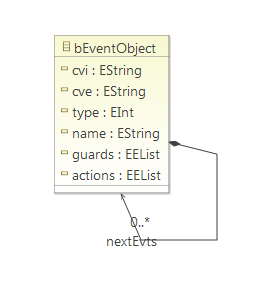
\includegraphics[width=0.5\textwidth]{img/ebo.PNG}
  \caption{The Data Structure of bEventObject}
  \label{fig:ebo}
\end{figure}

Recall that each event can references the control variable in the guards or actions, which controls the order that events take place. The \textbf{cvi} and \textbf{cve} in the bEventObject are short hand for control-variable-initial and control-variable-end. The cvi are used to determine which events that lead to the current event. Whereas the cve are used to determine which events that the current event can move into. They are derived from the guards and actions of the original event respectively (i.e. extracting the action/guard that references the control variable).

The \textbf{type} of a bEventObject is determined by the name of event under consideration:
\begin{itemize}
	\item An event has a \textbf{recursive} type if the event name starts with \textbf{REC} (case insensitive).
	\item An event has a \textbf{call} type if the event name starts with \textbf{CALL} (case insensitive).
	\item An event has a \textbf{normal} type if it is not one of the above cases.
\end{itemize}


The \textbf{guards} of the bEventObject is derived according to the following rules:
\begin{itemize}
	\item For the event of any type, its guards that reference the control variable are not included.
	\item For the event of recursive or call type, its guards are not included.
	\item For the event of recursive or call type, Additional guards might be added from the event name, depending on whether there are guards appeared in the event name (see Section~\ref{subsec:issue}).  
\end{itemize}

The \textbf{actions} of the bEventObject is derived according to the following rules:
\begin{itemize}
	\item For the event of any type, its non-deterministic actions are not included, i.e. becomes\_such\_that assignment  and becomes\_in\_set assignment are eliminated when parsing the event actions.
	\item For the event of any type, its actions that reference the control variable are not included.
	\item For the event of recursive or call type, its actions is not included.
	\item For the event of recursive or call type, an additional action is added from the event name (see Section~\ref{subsec:issue}).  
\end{itemize}

For the \textbf{nextEvts} association of the bEventObject, they help the plug-in understand how the transition system progress (i.e. where an event moves to the next). An bEventObject \textbf{x} counts as the “next event” of target bEventObject \textbf{y} if it has the following property:
\begin{lstlisting}
	x.cvi = y.cve
\end{lstlisting}
Such event y is then add to the nextEvts list of the target event x.


\subsection{Processing Event with Recursive/Call Type}\label{subsec:issue}
The event that has the recursive (or call) type must follows the following naming convention, so that the plug-in knows how to process it:

\lstset{language=[68]Algol}
\begin{lstlisting}
	rec@call_signature@grds@self_destructed
\end{lstlisting}

The \textbf{rec} indicates this event is of recursive type. The \textbf{call\_signature} part shows the function call to be invoked by the event. It takes the format:
\lstset{language=[68]Algol}
\begin{lstlisting}
	call_name(in_parameters; out_parameters)
\end{lstlisting} 
This signature is easy to turn into an deterministic action, then add to the action list of bEventObject. 

Recall that the guards of recursive event is not include in the guards of the bEventObject, the reason is that we use the \textbf{grds} part of event name to show under which the recursive call is allowed to be invoked. In case that an recursive event has no guards, specify \textbf{NULL} in the grds part. 

Notice that it is possible that more than one event's name that has the same signature exists, where only the guards of these events differ. They show different outcomes when executing the same recursive call. Thus, they should be combined. The plug-in use \textbf{self\_destructed} part in the event name to control which event to display (i.e. among all related events for a recursive call, only one of them is displayed). 

Eventually, each event is able to be translated into an bEventObject and be glued through nextEvts association. Next, we illustrate the algorithms that translate bEventObjects into control flow graph (Section~\ref{}) and recursive algorithm (Section~\ref{}).


\subsection{Representing in Control Flow Graph} 
An intuitive diagram allows easier understanding of the algorithm, and is a prerequisite for modularizing complex algorithms. Therefore, we show how to construct a control flow graph from each Event-B machine by using bEventObjects.

%Def 2.
The control flow graph is defined as $C = (G, N_{start}, Act, L_{act}, Grd, L_{grd})$, where:
\begin{itemize}
	\item G is a graph $G = (N, E, S_g, T_g)$, where N is a set of nodes; E is a set of edges; $S_g : E \rightarrow N $ is the source function for edges; and $T_g : E \rightarrow N$ is the target function for edges.
	\item $N_{start}$ is the start node, such that $\nexists e \in E : T_g(e) = N_{start}$.
	\item $Act$ is a set of actions.
	\item $L_{act} : E \rightarrow Act$ is an action function.
	\item $Grd$ is a set of guards.
	\item $L_{grd} : E \rightarrow Grd$ is an guard function.
\end{itemize}

This graph describes the control flow of a recursive algorithm. The construction algorithm of such graph is the following:
\begin{algorithm}
  \caption{Representing Event-B Machine as Control Flow Graph
    \label{alg:cfg}}
  \begin{algorithmic}[1]
    %\Require{}
    \Statex
    \Function{toCFG}{$bEventObject$}
      \ForEach{event $e \in nextEvts $}
        \State
        \Call{toCFG}{e}
        %\If{$z_i \neq 0$}
        %  \Let{$\delta$}{$\delta + 1$}
        %\EndIf
      \EndFor
      \State \Return{$G$}
    \EndFunction
  \end{algorithmic}
\end{algorithm}


\subsection{Representing in Recursive Algorithm}

For example, pretty printing an bEventObject into a textual representation takes 3-steps, i.e. printing the bEventObject's guards, actions and nextEvts in order.

\section{Proof Obligations}
We think there are a set of proof obligations that could be generated to ensure that an Event-B machine can be translated into a recursive algorithm:
\begin{itemize}
	\item The control variable in the actions and guards of each event are different. (i.e. the event progress)
	\item The labels in the Event-B machine forms an acyclic graph.
	\item Only one event that does not have control variable in its guards (i.e. the start event).
	\item Only one event that does not have control variable in its actions (i.e. the end event).
	\item The control variable in the events' actions is deterministic (i.e. An Event always know which label it should move into).
	\item Recursive calls and external function call are legal (i.e. type checked, signature matched).
	\item If the out label associates with more than one event, all these events should have guard(s) presented. Moreover, these guards should not overlapped and eventually converge.
\end{itemize}

\newpage
\section{Case Study}

\subsection{Binary Search Algorithm}
The first case study targets the binary search algorithm developed in the Event-B machine (a part of the machine is displayed in Fig~\ref{fig:mac}).
\begin{figure}[!h]
  \centering
\begin{minipage}{1.0\linewidth}
  \begin{minipage}{0.5\linewidth}
$
\begin{Bcode}
\Bevent {m1}	\quad \BRevent {find}\\
		\quad \Bkeyword{WHEN}\\
			\quad\quad { grd1 }:{ l=start }\\
			\quad\quad { grd2 }:{ lo=hi }\\
			\quad\quad { grd3 }:{ t(lo)=val }\\
		\quad \Bkeyword{WITNESSES}\\
			\quad	\quad{ j }:{ j=lo }\\
		\quad \Bkeyword{THEN}\\
			\quad\quad { act1 }:{ l:= end }\\
			\quad\quad { act2 }:{ ok:= TRUE }\\
			\quad\quad { act3 }:{ i:= lo }\\
		\quad \Bkeyword{END}
                \end{Bcode}$
\end{minipage} \begin{minipage}{0.5\linewidth}
$
\begin{Bcode}
\Bevent {m3} 	\quad \BRevent {find}\\

		\quad \Bkeyword{WHEN}\\
			\quad\quad { grd1 }:{ l=middle }\\
			\quad\quad { grd3 }:{ t(mi)=val }\\

		\quad \Bkeyword{WITNESSES}\\
			\quad \quad { j }:{ j=mi }\\
		\quad \Bkeyword{THEN}\\
			\quad\quad { act1 }:{ l:= end }\\
			\quad\quad { act2 }:{ ok:= TRUE }\\
			\quad\quad { act3 }:{ i:= mi }\\

			
		\quad \Bkeyword{END}
  
\end{Bcode}
$
\end{minipage}\end{minipage}


\begin{minipage}{1.0\linewidth}
\begin{minipage}{0.5\linewidth}
 $                \begin{Bcode}
\Bevent {m2} 	\quad \BRevent {fail}\\
		\quad \Bkeyword{WHEN}\\
			\quad\quad { grd1 }:{ l=start }\\
			\quad\quad { grd2 }:{ lo=hi }\\
			\quad\quad { grd3 }:{ t(lo)\neq val }\\
		\quad \Bkeyword{THEN}\\
			\quad\quad { act1 }:{ l:= end }\\

			\quad\quad { act2 }:{ ok:= FALSE }\\

		\quad \Bkeyword{END}
                \end{Bcode}
$

\end{minipage}
\begin{minipage}{0.5\linewidth}
$
\begin{Bcode}
\Bevent {split}\\		\quad \Bkeyword{WHEN}\\
			\quad\quad { grd1 }:{ l=start }\\

			\quad\quad { grd2 }:{ lo< hi }\\
		\quad \Bkeyword{THEN}\\
			\quad\quad { act1 }:{ l:= middle }\\
			\quad\quad { act2 }:{ mi:= (lo + hi)/ 2 }\\

		\quad \Bkeyword{END}
                \end{Bcode}
$
\end{minipage}
\end{minipage}

\noindent
\begin{minipage}{1.0\linewidth}\begin{minipage}{0.6\linewidth}
$
\begin{Bcode}

\Bevent {REC@rightsearchOK}	\quad \BRevent {find}\\
		\quad \Bkeyword{ANY}\quad { j }\\
		\quad \Bkeyword{WHERE}\\
			\quad\quad { grd1 }:{ l=middle }\\

			\quad\quad { grd2 }:{ val >  t(mi) }\\
			\quad\quad { grd3 }:{ j\in mi+1\upto hi }\\
			\quad\quad { grd4 }:{ t(j)=val }\\
			\quad\quad { grd5 }:{ mi+1 \leq hi }\\
		\quad \Bkeyword{THEN}\\
			\quad\quad { act1 }:{ i:= j }\\

			\quad\quad { act2 }:{ ok:= TRUE }\\
		\quad \Bkeyword{END}
                \end{Bcode}
$
\end{minipage}
\begin{minipage}{0.6\linewidth}
$
\begin{Bcode}
\Bevent {REC@rightsearchKO}
	\quad \BRevent {fail}\\

		\quad \Bkeyword{WHEN}\\
			\quad\quad { grd1 }:{ l=middle }\\
			\quad\quad { grd2 }:{ val >  t(mi) }\\
			\quad\quad { grd4 }:{ \forall  j \qdot  j \in  mi+1\upto hi \limp  t(j)\neq  val }\\
			\quad\quad { grd5 }:{ mi+1 \leq hi }\\
		\quad \Bkeyword{THEN}\\
			\quad\quad { act2 }:{ ok:= FALSE }\\
		\quad \Bkeyword{END}
\end{Bcode}
$  
\end{minipage}
\end{minipage}
  \caption{Event-B machine developed for the Binary Search Algorithm}
  \label{fig:mac}
\end{figure}

\newpage

As described in Section~\ref{subsec:issue}, the event of recursive/call type need to follow a naming convention so that the plug-in knows how to process it. In this example, the \textbf{REC@rightsearchOK} and \textbf{REC@rightsearchKO} are event of recursive type.  Their event name has been shorten in the above machine. The REC@rightsearchOK is a shorthand for:
\begin{lstlisting}
	rec@binsearch(t,mi+1,hi,val;ok,result)@NULL@SELF_DESTRUCTED
\end{lstlisting} 
and the REC@rightsearchKO stands for:
\begin{lstlisting}
	rec@binsearch(t,mi+1,hi,val;ok,result)@val>t(mi) && mi+1<=hi
\end{lstlisting} 

% [123]
The result of our translation is two-fold. First, to help people comprehend the algorithm, the plug-in read in the Event-B machine and visualize it as in Fig~\ref{fig:pix}. This is done by translating an bEventObject into a format that can be recognize by the \textit{Dot} tool of \textit{GraphViz} \footnote{http://www.graphviz.org/}. In a nutshell, the plug-in draw a circle for each label, and the arrow between two circles indicates an event occurs. The guards of such event is put onto the arrow, and the event's actions are the text in the square box. 

\begin{figure}[!h]
  \centering
    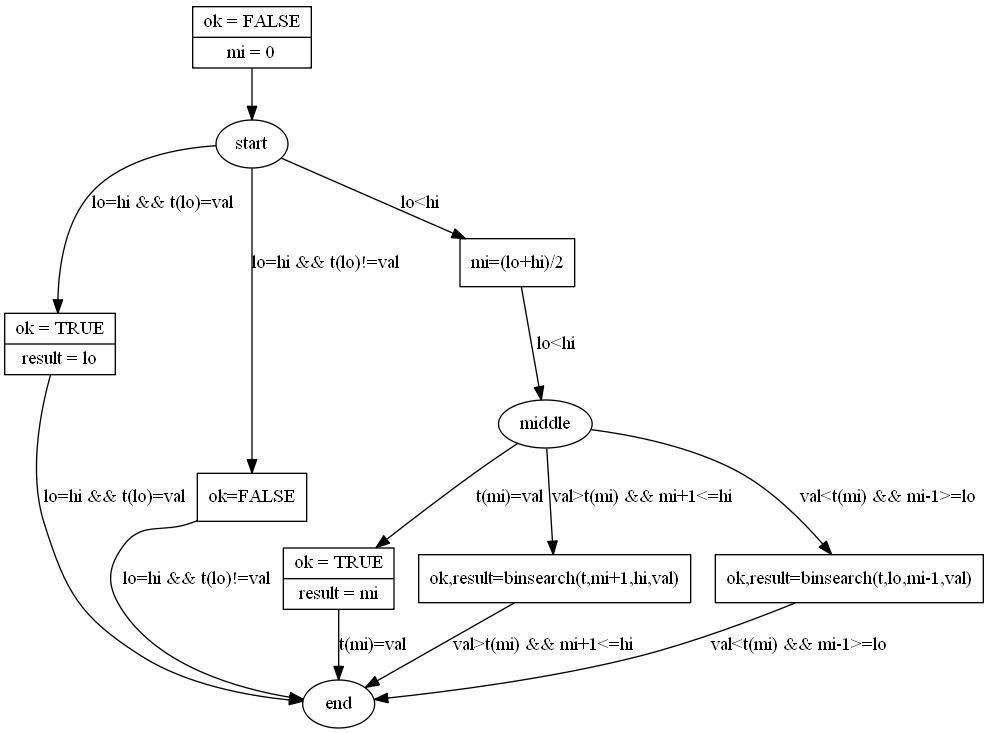
\includegraphics[width=0.8\textwidth]{img/pix.jpg}
  \caption{Visualized Representation of the Binary Search Algorithm}
  \label{fig:pix}
\end{figure}

Second, in Fig~\ref{fig:pix}, a textual representation of the binary search algorithm is given.
\begin{figure}[!h]
  \centering
    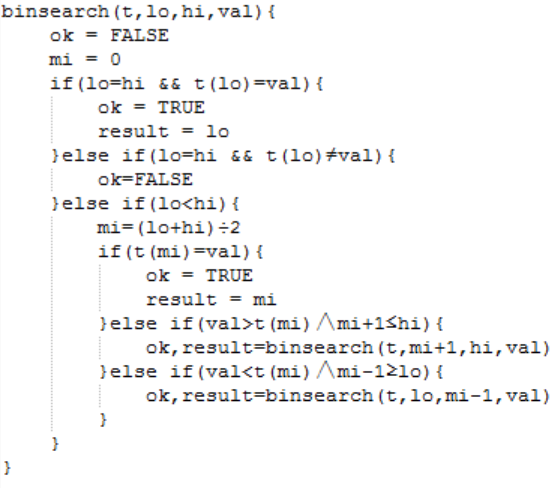
\includegraphics[width=0.5\textwidth]{img/alg.jpg}
  \caption{Textual Representation of the Binary Search Algorithm}
  \label{fig:alg}
\end{figure}








\end{document}

